\section{Taking a slice: diabetic patient analysis}\label{sec:diabetes}

The main conclusion to be taken away from the previous summative analysis is
that the dataset contains a huge amount of variation. Therefore, in order to
conduct more meaningful analysis, more homogenous subsets of the data must be
considered.

Classically, patients are categorised by age or condition. However, it has been
shown that doing so often gives an unrepresentative slice of
patients~\cite{Vuik2016}. In this section, the focus will be on the diabetic
population within the dataset despite this potential danger as it provides a
good example of condition-based slicing and is of interest to public health
groups.

Since diabetes is recorded only as a primary or secondary condition in the
dataset and is not distinguished by type, the diabetic population is considered
to be any instance where diabetes is present.

The ensuing analysis will provide evidence that the diabetic population is
increasing in the Cwm Taf area, and that, despite this, the relative resource
consumption by diabetic patients has been stagnant over the data period. It will
also be seen that this population holds too much variation to make meaningful 
conclusions about the population on the whole. However, by considering a subset
based on a condition such as this, there is a natural opportunity to compare
the subset with its complement; by considering the differences and similarities
between these two datasets a new dimension is added to the analysis.


\subsection{Distributions and summative statistics}%
\label{subsec:diabetes_distributions_statistics}

In much the same way as in Section~\ref{subsec:distributions_statistics}, taking
an overview of the key attributes provides some idea about how costs are
represented in the data.
Figures~\ref{fig:diabetes_no_spells_bar}~\--~\ref{fig:diabetes_netcost_kde} show
the same statistics as in the summative analysis though these figures have two
additional components: (a) in the case of bar charts, separate plots for overall
frequency and frequency density, and (b) a comparison with the non-diabetic
population on the same axes.

\begin{figure}[htbp]
    \centering
    \includegraphics[width=\imgwidth]{no_spells_bar/main.pdf}
    \caption{Bar chart for the number of spells associated with a patient in the
        presence of diabetes and not.}%
    \label{fig:diabetes_no_spells_bar}
\end{figure}

\begin{figure}[htbp]
    \includegraphics[width=\imgwidth]{los_bar/main.pdf}
    \caption{Bar chart for the total length of a spell in the presence of
        diabetes and not, clipped at 21 days. \textit{Maximum 705 days.}}%
    \label{fig:diabetes_los_bar}
\end{figure}

\begin{figure}[htbp]
    \centering
    \includegraphics[width=\imgwidth]{no_diag_bar/main.pdf}
    \caption{Bar chart for the maximum number of diagnoses in a spell in the
        presence of diabetes and not.}%
    \label{fig:diabetes_no_diag_bar}
\end{figure}

\begin{figure}[htbp]
    \centering
    \includegraphics[width=\imgwidth]{no_proc_bar/main.pdf}
    \caption{Bar chart for the total number of procedures in a spell in the
        presence of diabetes and not.}%
    \label{fig:diabetes_no_proc_bar}
\end{figure}

\begin{figure}[htbp]
    \centering
    \includegraphics[width=\imgwidth]{netcost_kde/main.pdf}
    \caption{Estimated probability density for the net cost of a spell in the
        presence of diabetes and not, clipped at \pounds12,500.}%
    \label{fig:diabetes_netcost_kde}
\end{figure}

\begin{figure}[htbp]
    \centering
    \includegraphics[width=\imgwidth]{age_bar/main.pdf}
    \caption{Bar chart for the age of patients in the presence of diabetes and
        not.}%
    \label{fig:diabetes_age_bar}
\end{figure}

\begin{table}[htbp]
    \vspace{-40pt}
    \resizebox{\imgwidth}{!}{%
        \begin{tabular}{llllll}
\toprule
{} &                     COST &                  NetCost &                       CRIT &                   DRUG &                  EMER \\
\midrule
mean &      2,801.26 (1,732.47) &      2,648.98 (1,647.00) &           -152.28 (-85.47) &         117.66 (70.98) &           1.49 (1.22) \\
std  &      4,755.10 (3,604.26) &      4,152.20 (3,019.53) &        1,543.66 (1,302.48) &        308.05 (314.59) &         18.94 (29.92) \\
min  &             10.91 (4.50) &             10.91 (4.50) &  -193,076.19 (-250,000.61) &          -0.24 (-0.57) &           0.00 (0.00) \\
1\%   &           140.16 (62.55) &           139.65 (62.55) &      -4,351.60 (-1,947.99) &            0.03 (0.00) &           0.00 (0.00) \\
25\%  &          493.10 (339.15) &          490.64 (338.67) &                0.00 (0.00) &           11.98 (6.70) &           0.00 (0.00) \\
50\%  &        1,242.98 (713.45) &        1,227.95 (709.32) &                0.00 (0.00) &          41.73 (18.97) &           0.00 (0.00) \\
75\%  &      3,191.26 (1,777.71) &      3,106.44 (1,756.90) &                0.00 (0.00) &         125.24 (55.12) &           0.00 (0.00) \\
99\%  &    21,380.12 (15,007.47) &    19,128.45 (13,414.48) &                0.00 (0.00) &      1,077.62 (790.91) &          12.06 (1.13) \\
max  &  273,450.30 (369,168.93) &  273,450.30 (369,168.93) &                0.00 (0.00) &  39,100.44 (63,430.52) &  1,274.44 (33,347.89) \\
\bottomrule
\end{tabular}

    }

    \vspace{3pt}

    \resizebox{\imgwidth}{!}{%
        \begin{tabular}{llllll}
\toprule
{} &                  ENDO &                    HCD &                   IMG &               IMG\_OTH &                     MED \\
\midrule
mean &         17.92 (21.49) &          30.88 (19.90) &         57.82 (30.12) &         37.11 (18.88) &         442.80 (336.51) \\
std  &         86.49 (93.10) &        282.12 (202.23) &       173.69 (139.60) &       137.35 (115.64) &         823.33 (723.61) \\
min  &           0.00 (0.00) &            0.00 (0.00) &           0.00 (0.00) &           0.00 (0.00) &             0.00 (0.00) \\
1\%   &           0.00 (0.00) &            0.00 (0.00) &           0.00 (0.00) &           0.00 (0.00) &             2.33 (0.00) \\
25\%  &           0.00 (0.00) &            0.00 (0.00) &           0.00 (0.00) &           0.00 (0.00) &           67.48 (42.63) \\
50\%  &           0.00 (0.00) &            0.78 (0.20) &           0.96 (0.07) &           0.00 (0.00) &         193.30 (125.47) \\
75\%  &           0.00 (0.00) &            8.47 (4.18) &          38.02 (5.68) &          14.20 (0.31) &         478.28 (364.67) \\
99\%  &       459.95 (452.73) &        538.46 (421.83) &       760.00 (496.25) &       622.04 (359.49) &     3,630.58 (2,853.92) \\
max  &  2,930.77 (11,855.95) &  31,451.98 (94,411.85) &  8,097.57 (46,708.66) &  8,097.57 (46,708.66) &  58,673.47 (116,449.90) \\
\bottomrule
\end{tabular}

    }

    \vspace{3pt}
    
    \resizebox{\imgwidth}{!}{%
        \begin{tabular}{llllll}
\toprule
{} &                     NCI &                    NID &                 OCLST &                   OPTH &                OTH \\
\midrule
mean &         -47.74 (-29.19) &         156.84 (88.22) &         23.79 (12.24) &        157.82 (160.10) &        3.03 (1.20) \\
std  &          111.85 (81.90) &        350.59 (230.71) &         86.84 (54.85) &        554.75 (471.42) &      17.35 (10.92) \\
min  &  -6,663.12 (-12,960.21) &            0.00 (0.00) &           0.00 (0.00) &            0.00 (0.00) &        0.00 (0.00) \\
1\%   &       -462.48 (-297.09) &            2.65 (1.84) &           0.00 (0.00) &            0.00 (0.00) &        0.00 (0.00) \\
25\%  &         -48.25 (-28.27) &          21.22 (14.52) &           0.00 (0.00) &            0.00 (0.00) &        0.00 (0.00) \\
50\%  &         -18.62 (-11.36) &          51.42 (31.14) &           1.83 (0.77) &            0.00 (0.00) &        0.00 (0.00) \\
75\%  &           -5.62 (-2.95) &         169.79 (76.98) &          12.30 (5.06) &            0.00 (0.04) &        0.25 (0.00) \\
99\%  &             0.00 (0.00) &      1,396.24 (916.69) &       356.95 (243.31) &    2,310.35 (2,083.16) &      94.37 (38.46) \\
max  &             0.00 (0.00) &  68,821.61 (84,374.21) &  5,155.60 (12,358.37) &  97,783.22 (51,651.76) &  787.82 (1,248.83) \\
\bottomrule
\end{tabular}

    }

    \vspace{3pt}

    \resizebox{\imgwidth}{!}{%
        \begin{tabular}{llllll}
\toprule
{} &            OTH\_OTH &                  OUTP &                    OVH &                   PATH &               PATH\_OTH \\
\midrule
mean &        2.09 (0.86) &           1.44 (0.49) &        578.90 (331.46) &          63.95 (33.31) &          42.12 (21.37) \\
std  &       14.90 (9.53) &         50.43 (23.29) &        983.48 (689.86) &        175.98 (129.62) &        159.98 (117.55) \\
min  &        0.00 (0.00) &           0.00 (0.00) &            0.00 (0.00) &            0.00 (0.00) &            0.00 (0.00) \\
1\%   &        0.00 (0.00) &           0.00 (0.00) &          43.77 (20.22) &            0.00 (0.00) &            0.00 (0.00) \\
25\%  &        0.00 (0.00) &           0.00 (0.00) &         107.56 (83.78) &            0.67 (0.00) &            0.00 (0.00) \\
50\%  &        0.00 (0.00) &           0.00 (0.00) &        230.05 (135.46) &           20.01 (3.72) &            0.74 (0.00) \\
75\%  &        0.00 (0.00) &           0.00 (0.00) &        663.48 (296.93) &          71.03 (28.55) &          35.24 (12.38) \\
99\%  &      79.99 (10.10) &           0.00 (0.00) &    4,548.67 (3,037.17) &        589.39 (370.62) &        486.22 (290.02) \\
max  &  787.82 (1,248.83) &  10,632.15 (9,989.54) &  57,647.29 (91,511.45) &  28,621.00 (70,008.12) &  28,621.00 (70,008.12) \\
\bottomrule
\end{tabular}

    }

    \vspace{3pt}

    \resizebox{\imgwidth}{!}{%
        \begin{tabular}{llllll}
\toprule
{} &                   PHAR &                   PROS &            RADTH &                 SECC &                    SPS \\
\midrule
mean &          58.15 (27.60) &          54.56 (39.22) &      0.50 (0.67) &          1.00 (0.86) &          21.49 (10.87) \\
std  &         124.21 (80.90) &        435.57 (331.92) &      7.24 (8.08) &        21.45 (27.94) &        190.25 (144.70) \\
min  &            0.00 (0.00) &            0.00 (0.00) &      0.00 (0.00) &          0.00 (0.00) &            0.00 (0.00) \\
1\%   &            0.02 (0.00) &            0.00 (0.00) &      0.00 (0.00) &          0.00 (0.00) &            0.00 (0.00) \\
25\%  &            3.75 (2.13) &            0.00 (0.00) &      0.00 (0.00) &          0.00 (0.00) &            0.00 (0.00) \\
50\%  &           16.13 (6.74) &            0.00 (0.00) &      0.00 (0.00) &          0.00 (0.00) &            0.00 (0.00) \\
75\%  &          71.52 (23.22) &            0.00 (0.00) &      0.00 (0.00) &          0.00 (0.00) &            0.00 (0.00) \\
99\%  &        479.20 (295.96) &    1,569.75 (1,263.77) &      0.00 (0.00) &        20.83 (10.42) &        799.16 (208.62) \\
max  &  14,812.14 (25,087.73) &  28,955.99 (33,930.70) &  227.64 (227.64) &  1,813.69 (2,177.74) &  14,008.47 (68,029.58) \\
\bottomrule
\end{tabular}

    }

    \vspace{3pt}

    \resizebox{\imgwidth}{!}{%
        \begin{tabular}{llllll}
\toprule
{} &                    THER &                     WARD &         TRUE\_LOS &        DIAG\_NO &        PROC\_NO \\
\midrule
mean &           57.23 (25.61) &          843.02 (460.63) &      6.07 (2.57) &    6.89 (3.14) &    2.05 (1.88) \\
std  &         207.44 (177.75) &      1,673.72 (1,165.64) &     12.55 (8.13) &    3.15 (2.72) &    2.58 (2.16) \\
min  &             0.00 (0.00) &              0.00 (0.00) &      0.00 (0.00) &    1.00 (0.00) &    0.00 (0.00) \\
1\%   &             0.00 (0.00) &              0.00 (0.00) &      0.00 (0.00) &    2.00 (0.00) &    0.00 (0.00) \\
25\%  &             0.18 (0.08) &             59.64 (9.04) &      0.00 (0.00) &    4.00 (1.00) &    0.00 (0.00) \\
50\%  &             7.53 (0.50) &          271.67 (136.97) &      1.00 (0.00) &    6.00 (2.00) &    2.00 (1.00) \\
75\%  &            47.84 (8.43) &          986.61 (429.02) &      7.00 (2.00) &    9.00 (4.00) &    3.00 (3.00) \\
99\%  &         684.15 (407.23) &      7,244.42 (4,855.75) &    57.00 (35.00) &  13.00 (13.00) &   12.00 (9.00) \\
max  &  17,643.81 (125,249.49) &  173,963.47 (203,854.11) &  705.00 (690.00) &  13.00 (13.00) &  43.00 (70.00) \\
\bottomrule
\end{tabular}

    }

    \thisfloatpagestyle{empty}
    \caption{Summative spell-level statistics for each of the key attributes. In
        each column the diabetic population's statistic in followed by the
        corresponding non-diabetic statistic in brackets.}%
    \label{tab:diabetes_summative}
\end{table}

\subsection{Pairwise correlation}\label{subsec:diabetes_correlation}

With an overview of how the key attributes are distributed in mind, as before,
it is a good idea to see how these attributes interact with one another. In
Figure~\ref{fig:diabetes_corr_heatmap}, the Pearson correlation coefficients
are shown between each of the pairs of the key attributes in the diabetic
population. Again, the attributes have been ranked in descending order according
to their summed absolute correlation coefficient (see
Definition~\ref{def:absolute_correlation}) to determine those with the highest
levels of interaction.

\begin{figure}[htbp]
    \makebox[\textwidth]{%
        \centering
        \includegraphics[height=.6\paperheight]{corr_heatmap/with_nums.pdf}
    }
    \caption{A heatmap of the pairwise correlation coefficients for the key cost
        attributes in diabetic patients. The attributes have been ordered
        according to their summed absolute correlation coefficient.}%
    \label{fig:diabetes_corr_heatmap}
\end{figure}

\begin{figure}[htbp]
    \makebox[\textwidth]{%
        \centering
        \includegraphics[height=.6\paperheight]{corr_difference/with_nums.pdf}
    }
    \caption{A heatmap of the difference in pairwise correlation coefficients
        between the diabetic and general populations. These attributes have been
        ordered according to the sum of their absolute values.}%
    \label{fig:diabetes_corr_difference}
\end{figure}


\subsection{Variation and relative importance}\label{subsec:diabetes_variation}

\begin{figure}[h]
    \centering
    \includegraphics[width=\imgwidth]{cost_variation/main.pdf}
    \caption{Bar chart showing the coefficient of variation \(C_{v}\) of each
        cost component, and the net and total costs, in the presence of diabetes
        and not.}%
    \label{fig:diabetes_variation}
\end{figure}

\begin{figure}[h]
    \centering
    \includegraphics[width=\imgwidth]{cost_contribution/main.pdf}
    \caption{Bar chart showing the average contribution of each cost component
        to the net cost of a spell in the presence of diabetes and not.}%
    \label{fig:diabetes_contribution}
\end{figure}

\begin{figure}[h]
    \centering
    \includegraphics[width=\linewidth]{cost_bubble_plot/main.pdf}
    \caption{A bubble plot showing a comparison between the diabetic and
        non-diabetic populations' average contribution to the net cost of a
        spell along the vertical, and the coefficient of variation for that
        component as the size of its marker.}%
    \label{fig:diabetes_bubble_plot}
\end{figure}

\subsection{Resource consumption}\label{subsec:diabetes_resources}

\begin{itemize}
    \item Only plots not showing all data points
    \item Discussion on instrinsic error and misrepresentation vs.\ evolving
        patterns
    \item Seasonal effect; metrics and statistical tests?
    \item Summary of each plot and final conclusions
\end{itemize}

\begin{figure}
    \centering
    \includegraphics[width=\imgwidth]{admissions/main.pdf}
    \caption{Monthly averages for the proportion of daily admissions presenting
        diabetes. Fitted with a linear least-squares regression model.}%
    \label{fig:admissions}
\end{figure}

\begin{figure}
    \centering
    \includegraphics[width=\imgwidth]{los_time/main.pdf}
    \caption{Monthly averages for the average length of a diabetic patient's
        spell given their admission date. Fitted with a linear least-squares
        regression model.}%
    \label{fig:los_time}
\end{figure}

\begin{figure}
    \centering
    \includegraphics[width=\imgwidth]{netcost_proportions/main.pdf}
    \caption{Monthly averages for the proportion of daily net cost spending
        toward diabetic patients given their admission date. Fitted with a
        linear least-squares regression model.}%
    \label{fig:netcost_proportions}
\end{figure}
